\documentclass[a4paper, 12pt]{article}

\usepackage{dblfnote}
\usepackage[perpage]{footmisc}
\usepackage{indentfirst}
\usepackage{framed}
\usepackage{tikz}
\usepackage{listings}[language=Python]
\usepackage{float}
\usepackage{subcaption}
\usepackage[square,numbers]{natbib}
%\usepackage{multicol}

\usepackage{setspace}
%\usepackage[skip=2mm, indent=17pt]{parskip}
\onehalfspacing
%\doublespacing


% Custom colors
\usepackage{color}

%\setcounter{secnumdepth}{0}

\usepackage[top=3cm, bottom=3cm, left = 2cm, right = 2cm]{geometry} 
\geometry{a4paper} 
\usepackage{url}
\usepackage{graphicx} 
\usepackage{amsmath,amssymb}  
\usepackage[hidelinks]{hyperref}
\usepackage[labelformat=empty]{caption}
\usepackage{xepersian}
\settextfont{XB Yas}
\usepackage[utf8]{inputenc}

%\usepackage{xepersian}

\DeclareFixedFont{\ttb}{T1}{txtt}{bx}{n}{12} % for bold
\DeclareFixedFont{\ttm}{T1}{txtt}{m}{n}{12}  % for normal

\definecolor{deepblue}{rgb}{0,0,0.5}
\definecolor{deepred}{rgb}{0.6,0,0}
\definecolor{deepgreen}{rgb}{0,0.5,0}

\newcommand\pythonstyle{\lstset{
		language=Python,
		basicstyle=\ttm,
		morekeywords={self},              % Add keywords here
		keywordstyle=\ttb\color{deepblue},
		emph={MyClass,__init__},          % Custom highlighting
		emphstyle=\ttb\color{deepred},    % Custom highlighting style
		stringstyle=\color{deepgreen},
		frame=single,                         % Any extra options here
		showstringspaces=false
}}


% Python environment
\lstnewenvironment{python}[1][]
{
	\pythonstyle
	\lstset{#1}
}
{}

% Python for external files
\newcommand\pythonexternal[2][]{{
		\pythonstyle
		\lstinputlisting[#1]{#2}}}

% Python for inline
\newcommand\pythoninline[1]{{\pythonstyle\lstinline!#1!}}




\begin{document}	
	\noindent
	\begin{minipage}[c]{5cm}
		\baselineskip=.7cm
		\begin{flushright}
			درس : مباحث ویژه در داده‌کاوی
			\\
			دانشجو :
			امیرمحمد خرازی
			\\
			شماره دانشجویی :
			40152521002 
			\\
			استاد درس :  
			\href{mrezghi.ir}{دکتر منصور رزقی آهق}
		\end{flushright}
	\end{minipage}
	\hfill
	\begin{minipage}[c]{3cm}
		\begin{center}
			\href{modares.ac.ir}{
				
\includegraphics[width=2cm]{logo.png}}
		\end{center}	
	\end{minipage}
	\\[1mm]
	\hrule depth .5mm \relax
	\begin{flushright}
		تمرین اول
		\hfill
		دانشکده علوم ریاضی ، گروه علوم کامپیوتر، گرایش داده‌کاوی
		\\
		\vspace{5mm}
		گیت‌هاب درس (
		\href{https://github.com/A-M-Kharazi/Special-Topics-in-DataMining-TMU.git}{لینک}
		)
		\hfill
		گیت‌هاب این تمرین (
		\href{https://github.com/A-M-Kharazi/Special-Topics-in-DataMining-TMU/tree/main/Homeworks/HW%201}{لینک}
		)
	\end{flushright}
	
	\hrule depth .5mm\relax
	
	%\tableofcontents
	%\newpage
	\section*{پرسش ۱ : }
	نشان دهید 
	\lr{k-means}
	یک روند کاهشی است.
	
	\vspace{5mm}
	پاسخ :
	
	الگوریتم 
	\lr{k-means}
	بطور خلاصه به شکل زیر عمل می‌کند : ابتدا ما تعداد $k$
	را برای این الگوریتم مشخص می‌کنیم (روش‌هایی نیز وجود دارند که خودشان این $k$ را پیدا می‌کنند). الگوریتم 
	\lr{k-means}
	مورد نظر ما، همان الگوریتمی است که در کتاب 
	\cite{book}
	صفحه 
	372
	معرفی شده است. بعد از مشخص کردن این $k$، الگوریتم $k$ مرکز تصادفی تولید می‌کند 
	($t = 0$)
	. در حال حاضر تعداد 
	$k$
	تا
	خوشه داریم که خالی هستند (مراکز خوشه ها می‌توانند نقاطی فرضی باشند که در نمونه‌های واقعی ما وجود ندارند). سپس در هر گام دو کار انجام می‌دهیم  : 
	\begin{enumerate}
		\item 
		هر داده‌ را به یک خوشه ارتباط می‌دهیم :  
		
		برای اینکار ابتدا
		\textbf{فاصله} 
		هر داده تا مرکز خوشه مرحله قبل را محاسبه می‌کنیم. 
		سپس داده را به خوشه‌ای متعلق می‌کنیم که با مرکز آن در گام قبلی، 
		\textbf{کمترین}
		فاصله را داشته باشد. یعنی بطور مثال اگر 
		$k=3$
		باشد، برای هر داده در هر مرحله از الگوریتم، فاصله داده تا مرکز خوشه (در مرحله قبل) را محاسبه می‌کنیم ، یعنی در این مثال ۳ فاصله محاسبه می‌شود، سپس داده را به خوشه ای که نماینده آن کمترین فاصله را با داده دارد، مرتبط می‌کنیم.
		\item
		مراکز جدید را برآورد می‌کنیم :
		
		بعد از مشخص شدن تکلیف هر داده در این مرحله (در بخش قبل)، خوشه‌ها و اعضای آن‌ها مشخص هستند. کافی است نماینده خوشه ، که در اینجا ما آن‌را میانگین اعضای خوشه می‌گیریم، مشخص شود. برای اینکار کافی است از داده‌های عضو هر خوشه میانگین بگیریم و مرکز جدید خوشه را بدست آوریم. 		
	\end{enumerate}  
	
	مراحل بالا را تا زمانی که همرایی رخ دهد ادامه می‌دهیم. یعنی می‌توانیم یک شرط روی آن داشته باشیم که اگر مراکز خوشه‌ها تفاوت چندانی نکردند (در گام‌های متوالی)، آنگاه الگوریتم به بهینه خود رسیده است. این الگوریتم یک روش تکراری است که با مراکز خوشه تصادفی شروع به کار میکند و هر بار اعضای خوشه‌ها را بدست آورده و مراکز جدید را تشکیل می‌دهد تا به بهین برسد (یعنی مراکز تغییر زیادی نداشته باشند). اگر اشتباه نکنم، بهینه 
	\lr{k-means}
	خیلی خوب نیست و انتخاب نقاط تصادفی اولیه برای مراکز روی آن تاثیر دارد ، لذا چندین بار این الگوریتم را اجرا میکنند و بهترین را به عنوان جواب در نظر می‌گیرند.
	
	
	دو نکته در بالا حائز اهمیت است : 
	فاصله و کمترین . 
	همانطور که  از تعریف و رنود الگوریتم 
	\lr{k-means}
	مشخص است، از آنجایی که ما فاصله را به عنوان معیاری برای شباهت و عدم شباهت داده‌ها مشخص کردیم، هر چه فاصله یک داده از هم دیگر دور باشد، کمتر شبیه هستند و برعکس، هر چه فاصله کم باشد، بیشتر شبیه هستند. هدف ما این است که داده‌هایی که شبیه هم هستند در یک خوشه قرار بگیرند و داده‌هایی که شبیه نیستند از هم دور باشند.  برای اینکار، مجبوریم حداقل فاصله را در نظر بگیریم. لذا این الگوریتم، یک روند کاهشی دارد بدین صورت که در هر مرحله تلاش می‌کند فاصله داده تا مرکز خوشه مورد نظرش را کمینه کند.  لذا هدف بهینه سازی الگوریتم
	\lr{k-means}
	کمینه کردن مجموع فاصله‌ها است یعنی :
	\[
	C^\star = \min SSE(C)
	\]
	که در این تابع هدف، 
	$SSE$
	برابر 
	\lr{Sum of Squared Error}
	است و بصورت زیر محاسبه می‌شود:
	\[
	SSE(C) = \sum\limits_{i=1}^{k}\sum\limits_{x_j \in C_i} distance(x_j, \mu_i) \hspace{2cm}\mu_i = \frac{1}{|C_i|}\sum\limits_{x_j \in C_i}x_j
	\]
	که این فاصله را می‌توانیم 
	نرم ۱ ، نرم ۲ یا غیره در نظر بگیریم که در پرسش دوم این مسئله بررسی می‌شود.
	
	پس بطور خلاصه، در الگوریتم 
	\lr{k-means}
	هدف پیدا کردن مجموعه خوشه است که عناصر شبیه به هم در یک خوشه باشند. شباهت هر عنصر با خوشه یعنی شباهت عنصر با نماینده خوشه که در 
	\lr{k-means}
	این نماینده، میانگین عناصر موجود در خوشه است. طبیعتا عناصری که به نماینده خوشه خود شبیه هستند، به یکدیگر نیز شبیه‌اند. 
	
	گفتیم که در هر مرحله از الگوریتم فاصله داده تا مرکز خوشه‌ها محاسبه می‌شود و داده را به خوشه‌ای می‌بریم که تا مرکز آن کمترین فاصله را داشته باشد. با این تفسیر در هر مرحله مرکز خوشه به داده‌های آن خوشه نزدیک‌تر می‌شود تا جایی که دیگر تغییری نمی‌کند. نزدیکتر شدن یعنی فاصله آن کاهش می‌یابد (ممکن است فاصله مرکز خوشه با یک داده در مرحله‌ای نسبت به مرحله قبلش بیشتر شود ولی مجموع این فاصله‌ها، یعنی فاصله هر داده تا مرکز خوشه‌اش، در هر مرحله نسبت به مرحله قبل کاهش می‌یابد). 

لذا با توجه به برداشت من از سوال، روند کاهشی در الگوریتم 
\lr{k-means}
را می‌توان بصورت بالا توضیح داد.
	
	
	
	
	\section*{پرسش ۲ : }
	روش 
	\lr{k-means}
	را با نرم یک و نرم 
	$l_p$
	به ازای 
	$p=4$
	بنویسید.
	
	\vspace{5mm}
	پاسخ :
	
	
	با توجه به الگوریتم 
	\lr{k-means}
	که در کتاب 
	\cite{book}
	صفحه  373
	آورده شده است، و همچنین توضیحاتی که در پرسش قبل آورده شده است، کافی است در هر مرحله، در هنگام محاسبه فاصله از نرم‌های گفته شده استفاده کنیم. یعنی در هر گام، در مرحله عضویت بخشیدن هر داده به یک خوشه، بجای محاسبه فاصله به روز 
	$L2$
	از روش‌های 
	$L1$
	یا
	$L_p$
	برای 
	$p=4$
	استفاده کنیم. فرض کنید 
	$x$
	و
	$y$
	هر دو متعلق به فضای $D$ بعدی باشند 
	($x,y \in \mathbb{R}^D$)
	. آنگاه 
	$distance(x,y)$
	را با توجه به نرم‌های زیر، بیان می‌کنیم :
	\begin{align*}
		L2-norm &\Longrightarrow distance(x,y) = \sqrt[2]{\sum\limits_{i=1}^{D} (x_i - y_i)^2}
		\\
		L1-norm &\Longrightarrow distance(x,y) = \sum\limits_{i=1}^{D} |x_i - y_i|
		\\
		L_p-norm(p=4) &\Longrightarrow distance(x,y) = \sqrt[p]{\sum\limits_{i=1}^{D} (x_i - y_i)^4}	
	\end{align*}
	البته در 
	$L2$
	و 
	$L_p$
	به جای 
	$(x_i - y_i)$
	باید قدر مطلق آن یعنی 
	$|x_i - y_i|$
	نوشته شود که چون توان ۲ یا توان ۴ باعث می‌شود جواب مثبت باشد (زیرا در حال محاسبه فاصله هستیم که فاصله همیشه مثبت است، یعنی نرم همیشه مثبت است) دیگر از قدر مطلق استفاده نکردیم. 
	
	در 
	\lr{k-means}
	معمولی که در فضای اقلیدسی از نرم ۲ برای محاسبه فاصله استفاده می‌کند بدین صورت عمل می‌کردیم:
	\begin{enumerate}
		\item 
		در مرحله 
		$(t = 0)$
		قرار داریم.
		ابتدا $k$ مرکز تصادفی تولید/انتخاب می‌کنیم.
		\item
		مرحله 
		$t = t + 1$
		، تعداد 
		$k$
		مجموعه خوشه خالی تولید می‌کنیم، یعنی مجموعه 
		$C_1, \dots, C_k$
		که همه آن‌ها خالی هستند.
		\item
		برای هر داده فاصله این داده تا مرکز هر خوشه را محاسبه کرده و خوشه‌ای که حداقل این فاصله را داشت، داده را دربر‌می‌گیرد. به زبان الگوریتمی‌تر، اگر 
		$x_j$
		داده مورد نظر ما باشد که می‌خواهیم تکلیفش را مشخص کنیم و 
		$i$
		روی خوشه‌های ما گردش می‌کند، آنگاه : 
		\begin{flalign*}
		j &= \min_i \left\{distance(x_j, center_i^{(t-1)})\right\}
		\\
		C_j &= C_j \cup \left\{x_j\right\}	
		\end{flalign*}
		\item
		با توجه به هر خوشه، مراکز جدید را می‌سازیم.
		پس خواهیم داشیت :
		$center_i^{(t)} = update(center_i^{(t-1)})$
		
		\item
		مرحله ۲ تا ۴ را تکرار می‌کنیم تا به شرط همگرایی برسیم.
	\end{enumerate}
	در الگوریتم بالا که الگوریتم 
	\lr{k-means}
	معمولیست، فاصله و نماینده خوشه‌ها می‌توانند نسبت به هم انتخاب شوند. در اینجا نماینده را مرکز خوشه در نظر گرفتیم . مرکز خوشه می‌تواند میانگین اعضای هر خوشه باشد اما لزومی نداریم که حتما از میانگین به عنوان نماینده خوشه استفاده کنیم؛ مثلا می‌توانیم از میانه استفاده کنیم. 
	
	در 
	$L2$
	انگار دنبال برآورد یک مدل گاوسی آمیخته هستیم . به نظرم با این تفسیر در 
	$L1$
	به دنبال برآورد یک مدل لاپلاس یا نمایی هستیم. 
	
	فرض کنیم داده‌های ما 
	$x_1,x_2,\dots,x_n$ 
	از توزیع گاوسی آمده باشند. براساس رابطه 
	\lr{Maximum Likelihood}
	برای تخمین پارامتر‌های مدل داریم :
	\begin{align*}
		f(x_1,x_2,\dots,x_n) = \frac{1}{\sqrt{2\pi\sigma^2}}\prod\limits_{i=1}^{n}\exp\left(-\frac{1}{2}\left(\frac{x_i - \mu}{\sigma}\right)^2\right)
	\end{align*}
که با 
	$\log$
	گرفتن آن را به جمع تبدیل کرده و ماکسیمم کردن آن با منفی کنار 
	$x_i$
	به مینیمم سازی تبدیل می‌شود که در نهایت مسئله را به کمینه کردن مجموع 
	$(x_i - \mu)^2$
	تبدیل می‌کند که این خودش همان مفهوم 
	$L2$
	است. به زبان دیگر :
	\begin{align*}
		\max \left\{-(\dots)\right\} \longleftrightarrow \min (\dots) \longleftrightarrow \min \sum\limits_{i=1}^{n} (x_i - \mu)^2
	\end{align*}
	این 
	$n$
	در حقیقت برای یک خوشه است. حالا اگر توزیع نمایی باشد بطور مشابه داریم :
	\begin{align*}
		f(x_1,x_2,\dots,x_n) = \frac{1}{\beta^n}\prod\limits_{i=1}^{n}\exp\left(\frac{x_i - \mu}{\beta}\right)
	\end{align*}
	که بطور مشابه خواهیم داشت :
	\begin{align*}
		\max \left\{-(\dots)\right\} \longleftrightarrow \min (\dots) \longleftrightarrow \min \sum\limits_{i=1}^{n}|x_i - \mu|
	\end{align*}
	در موارد بالا منظور از 
	$\dots$
	ها در مینیمم سازی یا ماکسیمم سازی عباراتی هستند که بعد از 
	$\log$
	گرفتن بدست آمده‌اند که تعداد زیادی از آن‌ها ثابت هستند و تاثیری در بهینه سازی ندارند لذا ما فقط جملاتی را در نظر می‌گیریم که بهینه‌سازی در آن‌ها موثر است.
	
	با این تفاسیر می‌توان 
	$L2$
	و
	$L1$
	را برای 
	\lr{k-means}
	تا حدی تصور کرد. در حالت 
	$L_4$
	یعنی زمانی که از نرم ۴ استفاده می‌کنیم مثل تابع گاوسی است که 
	$\left((x_i - \mu)^2\right)^2$
	شده است. یعنی اینگار آن را به توان ۲ رسانده ایم. این موارد شاید با تعابیر از آمار مثلا اگر متغیر تصادفی $X$ دارای توزیع گاوسی با پارامتر‌های 1 , 1  باشد، متغیر تصادفی 
	$X^2$
	دارای چه توزیعی است؛ قابل درک باشد. چون ممکن است حجم پاسخ به این سوال بیش از حد انتظار شود، بیشتر از این وارد مطلب نمی‌شوم. 
	
	لذا بطور خلاصه کافی است برای استفاده از نرم‌های دیگر، فاصله را با آن نرم‌ها در الگوریتم 
	\lr{k-means}
	حساب کنیم و چنانچه لازم دیدیم، از نماینده‌های بهتری برای خوشه‌ها استفاده کنیم. بصورت پیشفرض نماینده هر خوشه مرکز آن یا میانگین اعضای آن خوشه می‌باشد که بصورت 
	$\mu_i = \frac{1}{|C_i|}\sum\limits_{x_j\in C_i}x_j$
	محاسبه می‌شوند.
	
	
	نمونه‌های جدیدی از 
	\lr{k-means}
	برای این منظور ابداع شده‌اند :
	\begin{itemize}
		\item 
		 برای 
		$L1$
		،
		\lr{K-medians}
		ابداع شده است که مراکز را بجای میانگین، با میانه حساب می‌کند و خطا را برای زمانی که از 
		$L1$
		استفاده می‌کنیم، حداقل می‌کند (نسبت به زمانی که با میانگین و $L1$
		استفاده می‌کردیم
		) 
		.
		\item
		برای متر‌های دیگر (دلخواه و احتمالا 
		$L_4$
		)
		،
		\lr{k-medoids}
		ابداع شده است، این روش به نسبت 
		\lr{k-means}
		معمولی که از فاصله اقلیدسی 
		$L2$
		استفاده می‌کرد، پرقدرت تر است و به نویز و داده‌های پرت کمتر حساس است. عملا این روش یک کلی‌تر از 
		\lr{k-means}
		است.
	\end{itemize}
	روش این الگوریتم‌ها نیز نسبتا ساده است : 
	\begin{itemize}
		\item 
		برای 
		\lr{k-medians}
		، کافی است با 
		$distance$
		ای که قبل‌تر معرفی کردیم (برای 
		$L1$
		)
		و میانه داده‌ها عمل کنیم. برای میانه داده‌ها را مرتب کرده و آن‌هایی که وسط داده‌ها قرار دارند را به عنوان میانه می‌گیریم. اگر داده‌ها وسط نداشت، میانگین دو داده‌ها که در وسط هستند را به عنوان میانه می‌گیریم. 
		
		\item
		برای 
		\lr{k-medoids}
		: 
		یک نقطه واسط یا 
		\lr{medoids}
	 	،عضوی از یک خوشه است که میانگین عدم شباهت آن با بقیه اعضای خوشه، کمینه است (یعنی وسط‌ترین است). 
	 	  
		\begin{enumerate}
			\item 
			ابتدا 
			$k$
			نمونه را به عنوان نقاط واسط در نظر می‌گیریم (در قبل به صورت تصادفی 
			$k$
			میانگین را به عنوان مرکز تولید می‌کردیم
			). 
			لذا در اینجا مراکز اعضای واقعی هستند، یعنی خوشان از نمونه‌ها هستند.
			
			\item
			هر داده را به نزدیک ترین نقطه واسط 
			\lr{(medoid)}
			مرتبط می‌سازیم.
			\item
			برای هر داده‌ای که 
			\lr{medoid}
			نیست، فاصله ‌اش را با 
			\lr{medoid}
			خوشه‌اش حساب می‌کنیم (این مقدار را مثلا 
			$cost(m_i,o_j)$
			برای خوشه 
			$i$
			ام و داده 
			$j$
			ام در نظر بگیرید.
			)
			. 
			مجموع این هزینه‌ها (فاصله‌ها) را 
			$cost$
			می‌نامیم. 
			\item 
			نقطه دیگری را به عنوان نمونه واسط انتخاب می‌کنیم و هزینه را دوباره برای آن محاسبه می‌کنیم. برای مطلوب است که هزینه در هر گام، کمتر از گام قبلی باشد. اگر کمتر شد، آن را به عنوان نقطه واسط در نظر می‌گیریم.
			\item
			گام‌های ۲ تا ۴ را ادامه می‌دهیم تا الگوریتم همگرا شود.
			
		\end{enumerate}
		
	\end{itemize}
	طبیعی است که در هر نوع الگوریتم، از هر نوع متری برای اندازه‌گیری فاصله (نزدیکی) استفاده کنیم، از همان متر برای بهینه‌سازی نهایی الگوریتم استفاده خواهیم شد.
	 
	
	
	
	\section*{پرسش ۳ : }
	روش 
	\lr{EM}
	را با توزیع لاپلاس (به جای توزیع گاوسی) بنویسید و الگوریتم آن را با جزئیات بنویسید.
	
	
	\vspace{5mm}
	پاسخ :
	
	
	با توجه به کتاب 
	\cite{book}
	صفحه 381 ، معادله 
	\lr{(13.6)}
	با توجه به توزیع لاپلاس نوشته می‌شود. 
	
	\[
	f(x, \mu_i, b_i) = \frac{1}{2b}\exp\left(-\frac{|x - \mu_i | }{b}\right)
	\]
	 معادلات بعدی آن 
	 \lr{(13.7)}
	 ،
	 \lr{(13.8)}
	 و
	 \lr{(13.9)}
	 شبیه کتاب است. هر بار پارامتر‌های مدل برآورد می‌شود تا به بهین برسیم که همان 
	 \lr{MLE}
	 است. 
	 روند آن شبیه به همان  گاوسی است ولی در جا‌ هایی که 
	 مثلا در تخمین واریانس از 
	 $(x - \mu_i)^2$
	 استفاده می‌کردیم، در اینجا به 
	 $|x - \mu_i|$
	 تبدیل می‌شود.
	 
	 متاسفانه برای حل این سوال، خیلی فرصت کافی نداشتم و لذا پاسخ کاملی برای این سوال ارائه نداده‌ام.
	 
	


	\section*{پرسش ۴ : }
	
	بین بازه‌ی 
	$[0,10]\times [0,10]$
	نزدیک ۵۰۰ تا داده رندوم به صورت یکنواخت تولید کنید. سپس این داده‌ها را توسط الگوریتم‌های زیر خوشه‌بندی کنید.
	\begin{itemize}
		\item 
		روش سلسله مراتبی با نرم یک و 
		\lr{Complete-link}
		\item
		روش 
		\lr{EM}
		\item
		روش 
		\lr{DBSCAN}
	\end{itemize}
نتایج این روش‌ها را تحلیل کنید.


\vspace{5mm}
	پاسخ :
	
	جزئیات کامل کد نویسی این سوال، در کد‌های ارائه شده قابل مشاهده و بررسی می‌باشد. کد‌های این بخش را می‌توانید با عنوان 
	\lr{\pythoninline{Uniform Random Numbers Clustering}}
	در پوشه مربوطه بیابید. همچنین این کد‌ها در لینک‌هایی که در ابتدای این گزارش ارائه شده است نیز موجود می‌باشد. 

	فرض کنید اگر تعداد خوشه‌ها برابر ۲ باشد، نتایج زیر بدست می‌آید:
	
	
	
	\begin{figure}[H]
		\begin{subfigure}[t]{.4\textwidth}
			\centering
			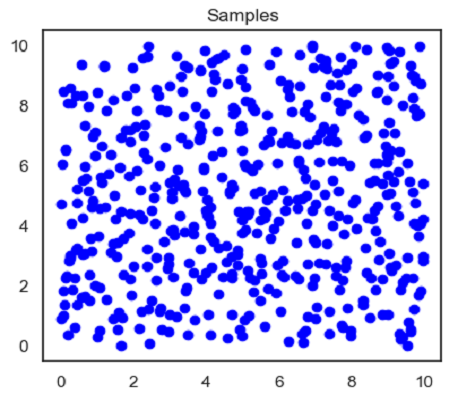
\includegraphics[width=\linewidth]{fig1.png}
			\caption{
			۵۰۰
			نمونه تصادفی	
		}
		\end{subfigure}
		\hfill
		\begin{subfigure}[t]{.4\textwidth}
			\centering
			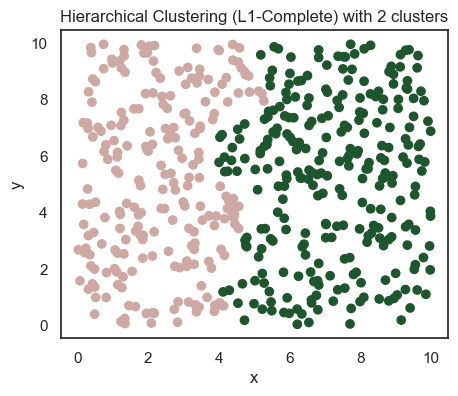
\includegraphics[width=\linewidth]{fig2.png}
			\caption{
			خوشه‌بندی با روش سلسه مراتبی نرم ۱ و 
			\lr{complete-link}	
		}
		\end{subfigure}
		
		\medskip
		
		\begin{subfigure}[t]{.4\textwidth}
			\centering
			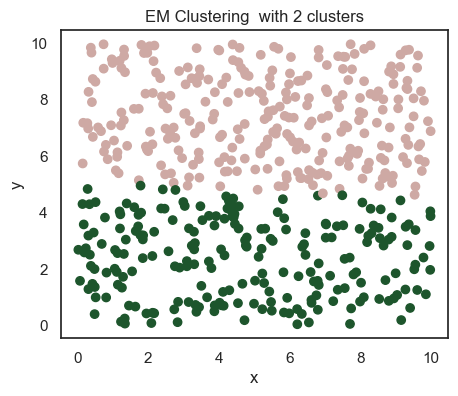
\includegraphics[width=\linewidth]{fig3.png}
			\caption{
			خوشه‌بندی با روش EM	
		}
		\end{subfigure}
		\hfill
		\begin{subfigure}[t]{.4\textwidth}
			\centering
			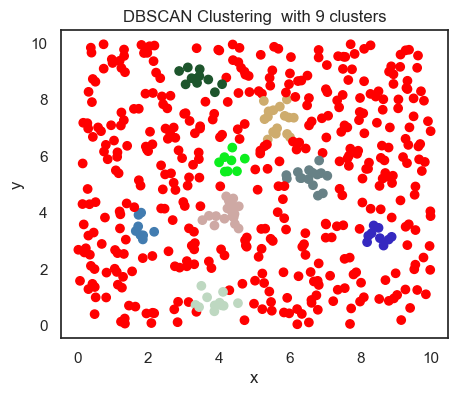
\includegraphics[width=\linewidth]{fig4.png}
			\caption{
			خوشه‌بندی با روش DBSCAN  با مقدار 
			$\epsilon = 0.5$
			و
			$min_samples = 8$	
		}
		\end{subfigure}
	\end{figure}
	
	
	
	
	
	
	

	\section*{پرسش ۵ : }
	داده‌های 
	\lr{IRIS}
	را دانلود کنید. 
	\begin{itemize}
		\item 
		این داده‌ها را با استفاده از الگوریتم‌های 
		\lr{k-means}
		،
		\lr{Hierarchical}
		،
		\lr{EM}
		و 
		\lr{DBSCAN}
		خوشه‌بندی کنید.
		\item
		این خوشه‌ها را توسط روش‌های مطرح شده (در کتاب قسمت 
		\lr{supervised/External}
		)
		ارزیابی کنید.

	\end{itemize}
	
	\vspace{5mm}
	پاسخ :
	
	جزئیات کامل کد نویسی این سوال، در کد‌های ارائه شده قابل مشاهده و بررسی می‌باشد. کد‌های این بخش را می‌توانید با عنوان 
	\lr{\pythoninline{IRIS Clustering}}
	در پوشه مربوطه بیابید. همچنین این کد‌ها در لینک‌هایی که در ابتدای این گزارش ارائه شده است نیز موجود می‌باشد.
	
	نتایج ارزیابی :
	\begin{latin}
Results : \\
$\bullet$ Hierarchical Clustering\\		
rand score : 0.8797315436241611\\
Normalized Mutual Information score : 0.7906785790830966\\
Fowlkes-Mallows score : 0.8237641241035158\\
$\bullet$ EM Clustering\\
rand score : 0.9574944071588367\\
Normalized Mutual Information score : 0.8996935451597475\\
Fowlkes-Mallows score : 0.9355985958131776\\
$\bullet$ DBSCAN Clustering\\
rand score : 0.7762863534675615\\
Normalized Mutual Information score : 0.5842137354876208\\
Fowlkes-Mallows score : 0.6887754949218047\\
$\bullet$ Kmeans Clustering\\
rand score : 0.8797315436241611
Normalized Mutual Information score : 0.7581756800057784
Fowlkes-Mallows score : 0.8208080729114153
	\end{latin}
مشاهده می‌شود که در اینجا الگوریتم 
$EM$
روی داده‌های آموزش
(داده‌های مشاهده شده)
 از همه بهتر جواب داده است. 	
	
	
	 نتایج خوشه‌بندی بصورت زیر است :
	
	\begin{figure}[H]
		
		\begin{subfigure}[t]{0.4\textwidth}
		\centering
		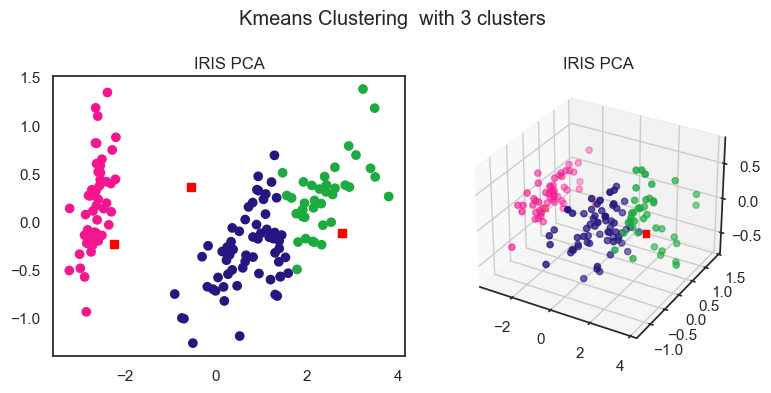
\includegraphics[width=\linewidth]{fig9.png}
		\caption{
			خوشه‌بندی با روش Kmeans  با مقدار 
			$\epsilon = 0.5$
			و
			$min_samples = 8$	
		}
	\end{subfigure}
	\hfill
	\begin{subfigure}[t]{.4\textwidth}
		\centering
		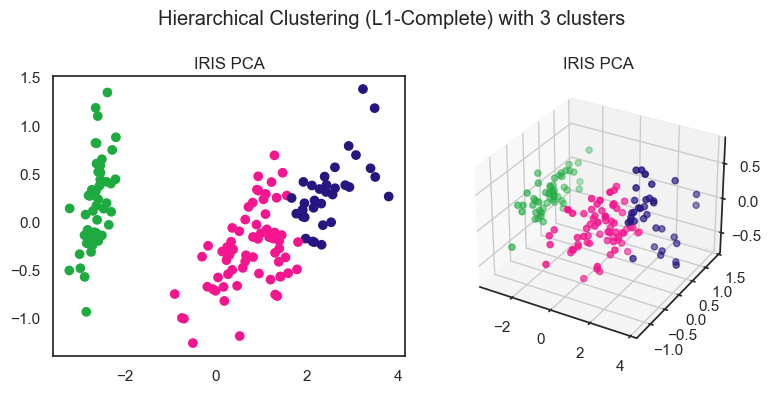
\includegraphics[width=\linewidth]{fig6.png}
		\caption{
			خوشه‌بندی با روش سلسه مراتبی نرم ۱ و 
			\lr{complete-link}	
		}
	\end{subfigure}
	
	\medskip
	
	\begin{subfigure}[t]{.4\textwidth}
		\centering
		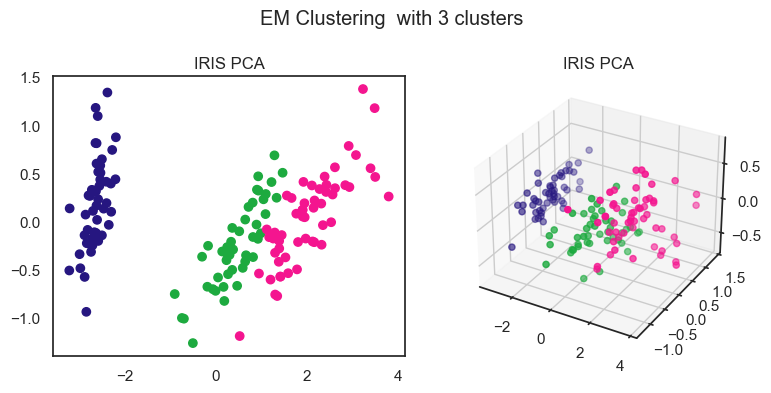
\includegraphics[width=\linewidth]{fig7.png}
		\caption{
			خوشه‌بندی با روش EM	
		}
	\end{subfigure}
	\hfill
	\begin{subfigure}[t]{.4\textwidth}
		\centering
		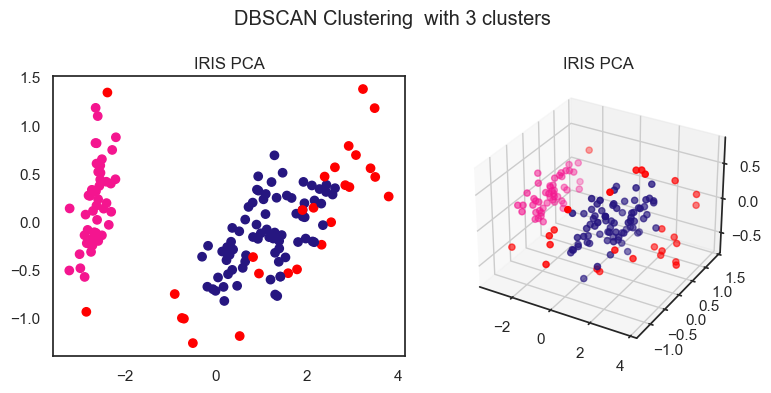
\includegraphics[width=\linewidth]{fig8.png}
		\caption{
			خوشه‌بندی با روش DBSCAN  با مقدار 
			$\epsilon = 0.5$
			و
			$min_samples = 8$	
		}
	\end{subfigure}
	
	\medskip
	
	\begin{subfigure}[t]{\textwidth}
		\centering
		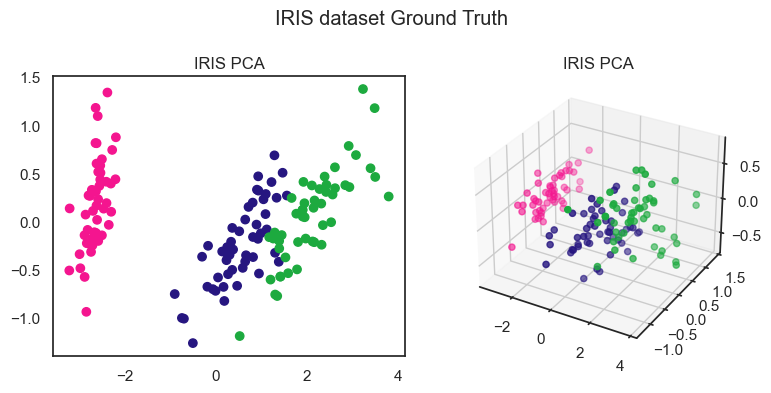
\includegraphics[width=\linewidth]{fig5.png}
		\caption{
			\lr{Ground Truth}
			داده‌های 
			IRIS	
		}
	\end{subfigure}

	\hfill
	
\end{figure}	
	
	
	
	
	
	
	
	\setLTRbibitems
	\makeatletter
	\bidi@AtBeginEnvironment{thebibliography}{\latinfont}
	\makeatother
	\bibliographystyle{unsrt} 
	\bibliography{ref.bib} 	
\end{document}


